\documentclass{article}
\usepackage{amsmath}
\usepackage[mathletters]{ucs}
\usepackage[utf8x]{inputenc}
\usepackage[margin=1.5in]{geometry}
\usepackage{enumerate}
\newtheorem{theorem}{Theorem}
\usepackage[dvipsnames]{xcolor}
\usepackage{pgfplots}
\pgfplotsset{compat/show suggested version=false}
\setlength{\parindent}{0cm}
\usepackage{graphics}
\usepackage{graphicx} % Required for including images
\usepackage{subcaption}
\usepackage{bigintcalc}
\usepackage{pythonhighlight} %for pythonkode \begin{python}   \end{python}
\usepackage{appendix}
\usepackage{arydshln}
\usepackage{physics}
\usepackage{tikz-cd}
\usepackage{booktabs} 
\usepackage{adjustbox}
\usepackage{mdframed}
\usepackage{relsize}
\usepackage{physics}
\usepackage[thinc]{esdiff}
\usepackage{fixltx2e}
\usepackage{esint}  %for lukket-linje-integral
\usepackage{xfrac} %for sfrac
\usepackage{hyperref} %for linker, må ha med hypersetup
\usepackage[noabbrev, nameinlink]{cleveref} % to be loaded after hyperref
\usepackage{amssymb} %\mathbb{R} for reelle tall, \mathcal{B} for "matte"-font
\usepackage{listings} %for kode/lstlisting
\usepackage{verbatim}
\usepackage{graphicx,wrapfig,lipsum,caption} %for wrapping av bilder
\usepackage{mathtools} %for \abs{x}
\usepackage[norsk]{babel}
\definecolor{codegreen}{rgb}{0,0.6,0}
\definecolor{codegray}{rgb}{0.5,0.5,0.5}
\definecolor{codepurple}{rgb}{0.58,0,0.82}
\definecolor{backcolour}{rgb}{0.95,0.95,0.92}
\pagecolor[rgb]{0.075,0.075,0.075} \color[rgb]{1,1,1} %TODO: Slett når ferdig%
\lstdefinestyle{mystyle}{
    backgroundcolor=\color{backcolour},   
    commentstyle=\color{codegreen},
    keywordstyle=\color{magenta},
    numberstyle=\tiny\color{codegray},
    stringstyle=\color{codepurple},
    basicstyle=\ttfamily\footnotesize,
    breakatwhitespace=false,         
    breaklines=true,                 
    captionpos=b,                    
    keepspaces=true,                 
    numbers=left,                    
    numbersep=5pt,                  
    showspaces=false,                
    showstringspaces=false,
    showtabs=false,                  
    tabsize=2
}

\lstset{style=mystyle}
\author{Oskar Idland}
\title{FYS2130 - Oblig 1}
\date{}
\begin{document}
\maketitle
\newpage

\section*{Oppgave 1}
\subsection*{a)}
\begin{figure}[h!]
  \centering
  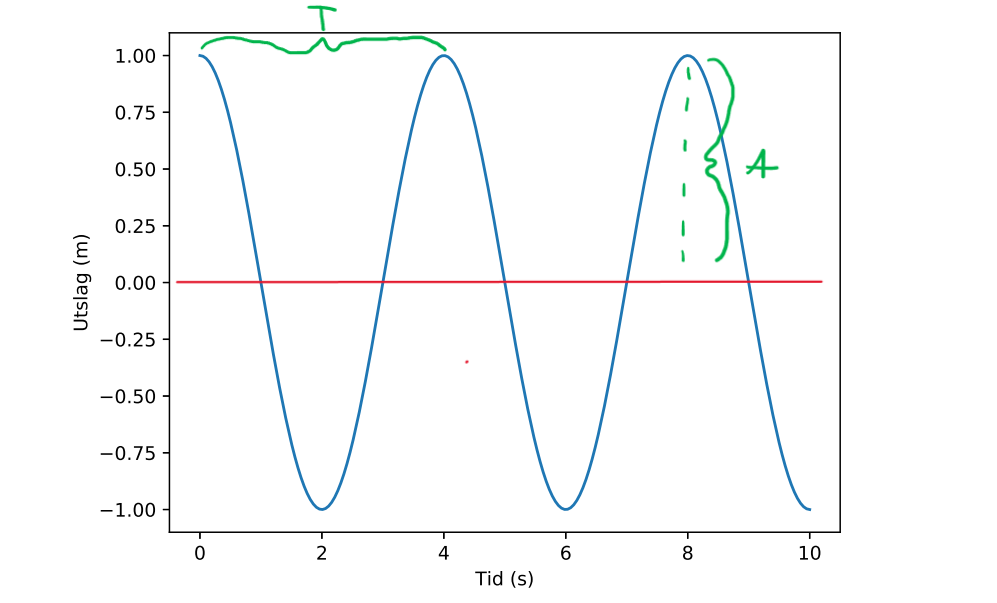
\includegraphics[scale = .5]{Figures/1.a.png}
  \caption{Oppgave 1a}
  \label{fig: 1a}
\end{figure}

Vi finner amplituden $A$ ved å se hvor høyt over likevektslinjen (ved y = 0) bølgetoppen kommer. Dette er $A = 0.5$ m. Periodetiden $T$ er hvor lang tid bølgen bruker på å gjennomføre én hel oscillasjon. Ettersom x-aksen er tid i sekunder trenger vi bare å se på avstanden på grafen. Her ser vi at $T = 4$. 

\subsection*{b)}
\begin{figure}[h!]
  \centering
  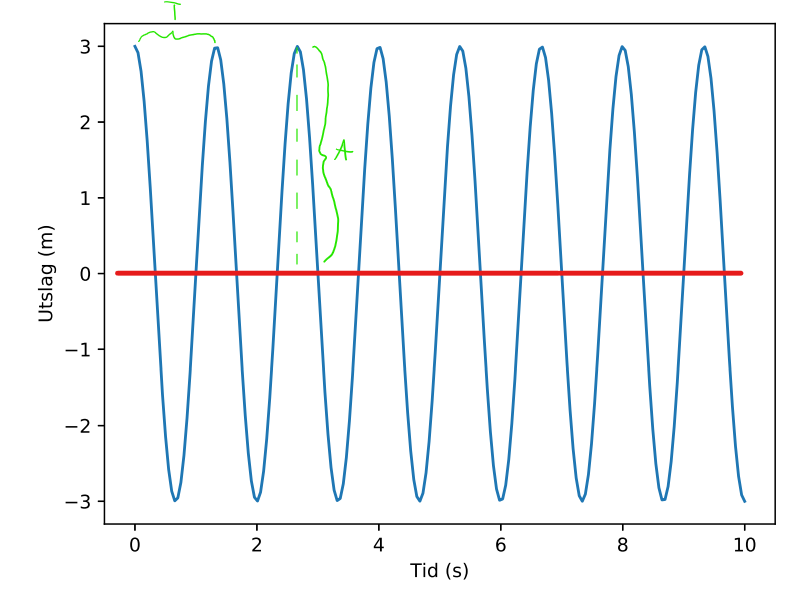
\includegraphics[scale = .5]{Figures/1.b.png}
  \caption{Oppgave 1b}
  \label{fig: 1b}
\end{figure}

Vi finner amplituden $A$ på samme måte og frekvensen $f = \frac{1}{T}$, finner $A = 3$ og $f = \frac{4}{3}$ 

\subsection*{c)}
\begin{figure}[h!]
    \centering
    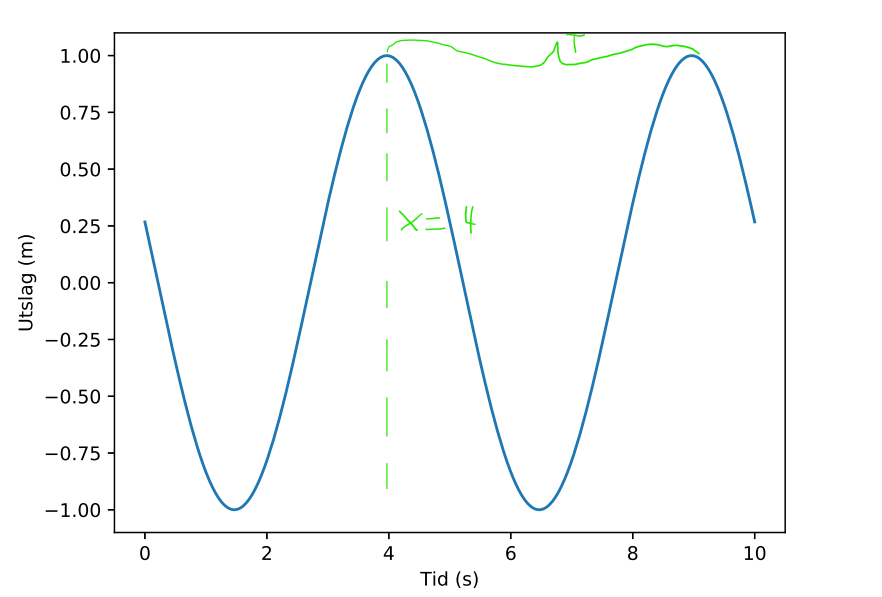
\includegraphics[scale = .5]{Figures/1.c.png}
    \caption{Oppgave 1c}
    \label{fig: 1c}
  \end{figure}
  
Vi vet at vinkelfrekvensen $ω = 2πf$. Vi må først finne $f$. Vi bruker samme metode som i b og finner periodetiden $T = 5$ som gir frekvens $f = \frac{1}{5}$ og $ω = 2πf = \frac{2π}{5}$. For å finne faseforskyvningen starter vi med å se på funksjonen når $t = 0$. Da er $y = 0.25$. Vi løser dette for det generelle tilfellet. 
\[
0.25 = \cos(ϕ)
\]
\[
 ϕ = \arccos (0.25)
\]

  
\section*{Oppgave 2}
\subsubsection*{a)}
For en harmonisk bevegelse kan posisjonen beskrives med en cosinus funksjon på formen
\[
x (t) = A \cos(ωt + ϕ)
\]
Da blir naturligvis 
\[
\ddot{x} = -ω^{2}x
\]
Videre bruker vi at $ΣF = ma = m \ddot{x}$ og at $ΣF = -kx$ for en fjær. 
\[
m \ddot{x} = -kx ⇒ - mω^{2}x = -kx
\]
\[
ω = \sqrt{\frac{k}{m}}
\]


\subsection*{b)}
Setter in $k = 8$, $m = 2$. 
\[
ω = \sqrt{\frac{8}{2}} = 2
\]
Da ser vi at $x$ blir følgende
\[
x = A \cos(2t + ϕ)
\]
For å løse for $A$ bruker vi at $x(0) = 0.4$
\[
0.4 = A \cos(ϕ) ⇒ A = \frac{0.4}{\cos(ϕ)}
\]
Vi setter dette inn i $\dot{x}(0) = -2$
\[
-2 = -2 \left( \frac{0.4}{\cos ϕ} \right)  \sin(ϕ)
\]
\[
1 = 0.4 \tan(ϕ)
\]
\[
ϕ = \arctan \left( \frac{5}{2} \right)  ≈ 1.19  , \quad A = \frac{0.4}{\cos  \left( \arctan \left( \frac{5}{2} \right)  \right) } ≈ 1.08
\]
Da får vi et utrykk for $x$ på formen
\[
x = 1.08 ⋅  \cos(2t + 1.19)
\]

\subsection*{c)}
Bruker Hook's lov for den potensielle energien. 
\[
E_p = \frac{1}{2}kx^{2} = 4 \left( 1.08 ⋅ \cos (2t + 1.19) \right) ^{2} = 4.67 ⋅ \cos ^{2}(2t + 1.19)
\]
\[
E_k = \frac{1}{2}m \dot{x}^{2} = 4.67 \sin ^{2} (2t + 1.19)
\]
\[
E = E_p + E_k = 4.67 ⋅ \cos ^{2}(2t + 1.19) + 4.67 \sin ^{2} (2t + 1.19)
\]
\[
E = 4.67 \text{ J}
\]
Løsningen viser at den mekaniske energien er konstant og dermed bevart. 

\newpage
\begin{figure}[h!]
  \centering
  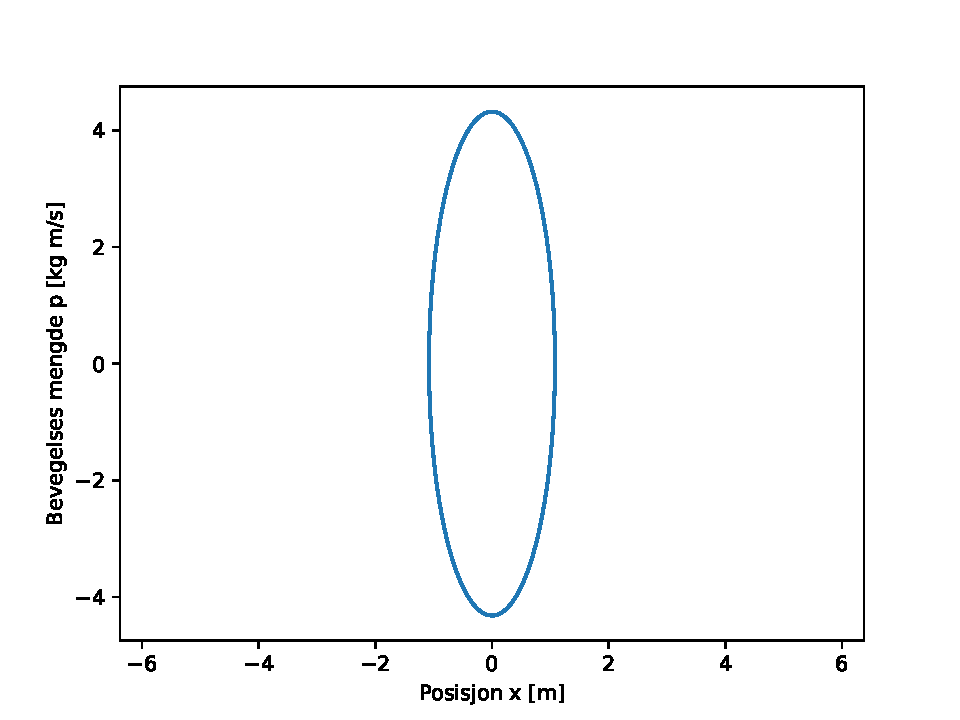
\includegraphics[scale = .5]{Figures/2_c.pdf}
  \caption{Plot av posisjon og bevegelsesmengde}
  \label{fig: 2c}
\end{figure}

\subsection*{d)}
Som vi ser i figur \ref{fig: 2d} Blir formen mye rundere når vi skalerer med $x_0$ og $v_0$. 
\begin{figure}[h!]
  \centering
  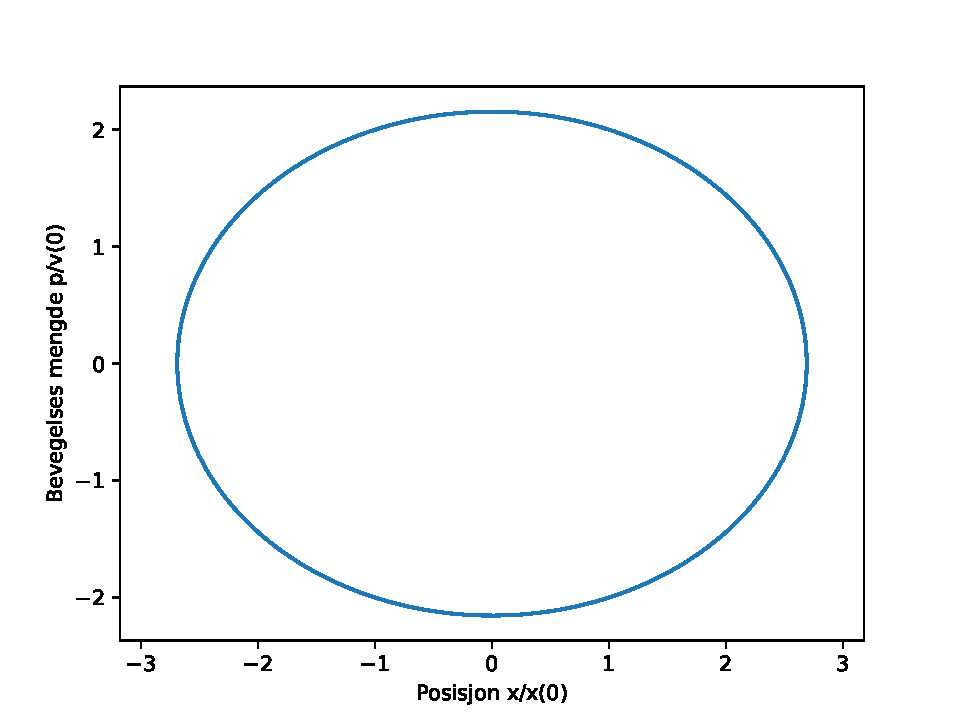
\includegraphics[scale = .5]{Figures/2_d.pdf}
  \caption{Plot av posisjon og bevegelsesmengde gjort dimensjonsløse ved å skalere med $x_0$ og $v_0$}
  \label{fig: 2d}
\end{figure}

\newpage
\section*{Oppgave 3}
Vi bruker det generelle uttrykket for en harmonisk bevegelse. 
\[
x = A \cos(ωt + ϕ), \quad \dot{x} = -ωx \quad \ddot{x} = -ω^{2}x
\]
\[
  m\ddot{x}\dot{x} = -  kx \dot{x} ⇒ m (-ω^{2})x -(ω)x = -kx (-ω)x
\]
\[
mω^{3} x^{2} = kωx
\]
\[
x = \frac{k}{mω^{2}}
\]



\end{document}